%\author{D. Crews}

\documentclass[12pt]{article}

\usepackage{amsmath}
\usepackage{graphicx}
\usepackage{bm}
\usepackage{mathabx}
\usepackage[margin=1.0in]{geometry}
\usepackage[english]{babel}
\usepackage{enumitem}
\usepackage{hyperref}
%\usepackage{roman}

\begin{document}
\title{\Large {\bf AA 321 | Aerospace Laboratory\\Lab Eight: Beam Vibrations}\\[1ex]
  University of Washington}
\date{\today}
\maketitle
%\tableofcontents

\section{A quick introduction to spectral analysis}\label{objs}
A ubiquitously utilized tool in vibration theory is spectral analysis. The main character is the Fourier series, whose central idea is that nearly any periodic waveform\footnote{That is, one satisfying minimally restrictive requirements called the Dirichlet conditions.} $f(x)$ can be decomposed into a series of sine and cosine functions, with convergence in the limit of an infinite number of terms. If the period of $f(x)$ is $L$ (that is, $f(x+L) = f(x)$), then
\begin{equation}
  f(x) = \frac{a_0}{2} + \sum_{n=1}^\infty a_n\cos(k_nx) + b_n\sin(k_nx)\label{fourier}
\end{equation}
is its Fourier series, where the coefficients $a_n$, $b_n$ depend on the particular function $f(x)$ and the frequencies $k_n=\frac{2\pi}{L}n$ are called ``wavenumbers'' (because they tell you the number of wave periods in a length $L$). This works because $\sin(x)$ and $\cos(x)$ form a complete set of orthogonal eigenfunctions for one-dimensional intervals. Let's now go further into this point.
\begin{figure}[h]
  \centering
  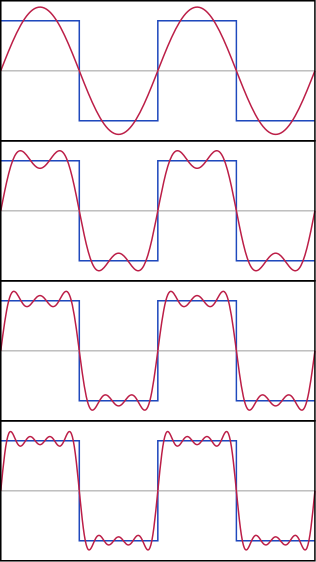
\includegraphics[width=0.19\textwidth]{fex}
  \caption{First four partial sums of the Fourier series for the rectangular wave [Wiki].}
\end{figure}
\newpage
The space that a function lives in is characterized by certain eigenfunctions (\textit{eigen} means ``own'' or ``inherent'', so read as ``characteristic functions'' of the space). The eigenfunctions are a \textit{basis} for the space. In the same way that vector components are found by projection onto basis vectors, a function's components are found by projecting onto the eigenfunctions (Fig. \ref{proj}). Just like basis vectors there are many possible choices of function basis. Of course, the most convenient ones are \textit{orthogonal} and the sines and cosines have just this property.
\begin{figure}[h]
  \centering
  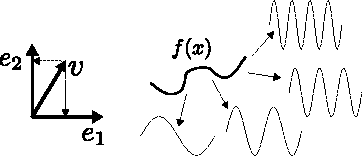
\includegraphics[width=0.75\textwidth]{fourier_projection}
  \caption{The Fourier coefficients $a_n$, $b_n$ of $f(x)$ are projections to an orthogonal basis, in the very same way that vector components of $v$ are projections onto basis vectors $e_1$ and $e_2$.}\label{proj}
\end{figure}

What do we mean by orthogonal functions? With vectors, orthogonality means that the measure of one against the other (using the inner product) is zero. For functions the notion of ``measuring one against the other'' is integration over the interval $x\in [0,L]$,
\begin{equation}
  \langle \sin(k_nx)|\sin(k_mx)\rangle = \int_0^L \sin\Big(\frac{2\pi}{L}nx\Big)\sin\Big(\frac{2\pi}{L}mx\Big)dx = \begin{cases} \frac{L}{2} & n=m\\
    0 & n\neq m\end{cases}
\end{equation}
making $\sin(k_nx)$ a family of orthogonal functions. This means that measuring one member against another gives zero, except for itself (try it for $L = 2\pi$ and $n=1$ to convince yourself). Using orthogonality, the coefficients in Eqn. \ref{fourier} are found by the integrals (the projections)
\begin{align}
  a_n &= \frac{2}{L}\int_0^L f(x)\cos(k_nx)dx,\label{f1}\\
  b_n &= \frac{2}{L}\int_0^L f(x)\sin(k_nx)dx.\label{f2}
\end{align}
If the math seems heavy, know that its generally more important to understand what these equations \textit{mean} than to actually do the calculations! There are many tools for calculations.

Now, the set of Fourier coefficients $a_n$, $b_n$ is called the \textit{spectrum} of the function and gives a measure of ``how much'' of the signal is composed of the frequencies $k_n$. For example, if you record yourself playing a note F\# on a guitar (370 Hz) and then calculate the coefficients $a_n$, $b_n$ of the waveform in the music file then there will be a huge peak around 370 Hz. Let's now go into some background on how Matlab will calculate these Fourier coefficients.
\newpage
\subsection{Complex form of the Fourier series}
Matlab does not calculate the integrals of Eqns. \ref{f1}-\ref{f2}, instead it approximates it using a little fancier theory. One can rewrite the Fourier series in the form
\begin{align}
  f(x) &= \sum_{n=-\infty}^\infty c_ne^{ik_nx},\\
  c_n &= \frac{1}{L}\int_0^Lf(x)e^{-ik_nx}dx\label{fourier2}
\end{align}
by using Euler's identity $e^{ix} = \cos(x) + i\sin(x)$. The notation $\sum_{n=-\infty}^\infty$ means to add all terms in the pairs $n=0, \pm 1, \pm 2, \pm 3, \cdots$. For example,
\begin{equation}
  f(x) = c_0 + c_{-1}e^{-ik_1x} + c_1e^{ik_1x} + c_{-2}e^{-ik_2x} + c_2e^{ik_2x} + \cdots.
\end{equation}
The relationship of these coefficients $c_n$ to the sine and cosine ones is that $c_n = \frac{1}{2}(a_n - ib_n)$. This form of the Fourier series is much more economical and the Fourier integral Eqn. \ref{fourier2} is generally easier to calculate than Eqns. \ref{f1}-\ref{f2}. If $f(x)$ is a real function, then all the imaginary parts will cancel out in the summation. Again, understanding what this equation means is more important than doing calculations with it. One is representing $f(x)$ in terms of its orthogonal components, the ``wiggles'' $b_n\sin(k_nx)$ and $a_n\cos(k_nx)$.

\subsection{The ``discrete Fourier transform''}
Suppose you are analyzing a music clip (or beam vibrations) and want to know which frequencies are present. Now the ``Fourier integral'' Eqn. \ref{fourier2} can't be done because the function $f(x)$ is not known. Instead, one has a \textit{time series} of data points, $f = [f_1, f_2, f_3, \cdots, f_N]$ with some sampling rate $\Delta x$. Using this time series, one can approximate Eqn. \ref{fourier2} using the simplest possible integral approximation, just adding up all of the integrand values,
\begin{align}
  c_n = \frac{1}{L}\int_0^Lf(x)e^{-ik_nx}dx \approx \frac{1}{L}\sum_{j=1}^Nf_je^{-ik_nx_j}\Delta x = \frac{\Delta x}{L}\sum_{j=1}^N f_je^{-ik_nx_j}
\end{align}
assuming a constant sampling rate. Because $L = N\Delta x$ and the phase factor simplifies like
\begin{equation}
  -ik_nx_j = -i\frac{2\pi}{L}n\Delta x j = -i\frac{2\pi}{N\Delta x}n\Delta x j = -i2\pi n\frac{j}{N}
\end{equation}
the result, called the discrete Fourier series coefficients, is usually written as
\begin{equation}
  c_n = \frac{1}{N}\sum_{j=1}^Nf_je^{-i2\pi n j/N}\label{fourier3}
\end{equation}
and is simply a summation over the data points with corresponding oscillator functions $e^{ix}$. It is a projection onto the orthogonal basis in the same way as before, just using a discrete set of data points! Now even a summation is pretty slow if the number of terms $N$ is large (like many millions for typical data files). Matlab calculates Eqn. \ref{fourier3} using a clever trick called the \textit{fast Fourier transform} or FFT, which breaks the summation down into smaller chunks. Fortunately, all you have to do is call \texttt{fft(X)} for \texttt{X} your data array!

\subsection{A quick Matlab FFT tutorial}
Here is a quick ``how to'' take an FFT in Matlab. Probably the most confusing part is assembling the correct vector of frequencies (note: there is a function in Python that does this for you...!). This example (Fig. \ref{fftex}) reads in a music file (a 9-second clip of a single C chord on the guitar) and analyzes its frequencies.
\begin{figure}[h]
  \centering
  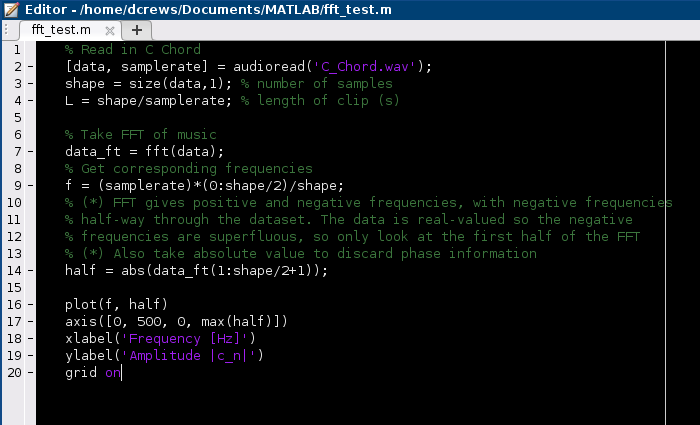
\includegraphics[width=0.5\textwidth]{matlab_fft_test}
  \caption{A quick test script to calculate the FFT a music clip.}\label{fftex}
\end{figure}
To find the sample frequencies, we need to form the wavenumbers $k_n = \frac{2\pi}{L}n$. The FFT calculates the wavenumbers up to a certain cut-off rate called the Nyquist frequency to avoid aliasing effects (which cause the result to look ``pixelly'', so that many video applications use special filters called ``anti-aliasing'' techniques). The Nyquist frequency is half of the sampling rate, so wavenumbers are built up to half of the total samples of the signal. Zooming in on the data with the \texttt{axis} command, Fig. \ref{cchord} is the resulting spectrum of the C-chord. Now try this on your beam vibration data!
\begin{figure}[h]
  \centering
  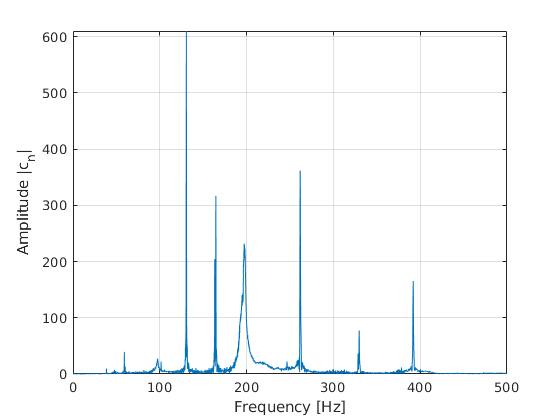
\includegraphics[width=0.5\textwidth]{woop}
  \caption{Component frequencies of the C-chord clip. The four notes played were the chord tonic C (131 Hz), then E (165 Hz), G (196 Hz), and finally the octave tonic C (262 Hz). Note that the octave is exactly twice the frequency of the original C! The spike at 393 Hz (G) is a \textit{harmonic} and was not actually played.}\label{cchord}
\end{figure}

\end{document}